\section{Related Work}
3D reconstruction and modeling from a single image has been extensively studied as the problem of \emph{shape from monocular cues}, including shadings~\cite{shapefromshadingsurvey}, focuses~\cite{shapefromdf1,shapefromdf2}, and textures~\cite{Aloimonos1988}. 
These methods usually recover 2.5D surfaces from 2D images. 
Learning-based approaches, especially deep learning methods, can acquire more complicate priors by learning from datasets and recover much more complete 3D shape from a single image.
 
\subsection{General Learning Approaches}
As far as we known, early work of learning approaches can be traced back to \cite{Hoiem2007} and \cite{learn3D2007}. These methods learn to segment and classify regions in image and finally produce 3D scene by folding the 2D image.
%
More recent techniques break down the problem to two stages\cite{Su:2014,jointimgshape}. One is to retrieve shape components from a large dataset, and the other is to assemble the components and deform the assembled shape to fit the observed image. These methods need to segment the shape into components for the database.
%
However, shape retrieval from images itself is an challenging problem due to the loss of information during 3D-to-2D projection. 
\cite{imgrecon15} avoid the retrieval step by learning a deformable 3D shape for each category and learn to predict deformation from input image for these specific categories.
%
%These learning approaches are relatively early.
%A more ideal solution would be to directly learn 3D shapes from single images under an end-to-end framework.
\begin{figure*}[htbp]
	\centering
	\includegraphics[width=\linewidth]{img/net/net}
	\caption{The cycle regularization implemented along with networks: (a) is the implementation with AtlasNet\cite{atlasnet}. $f$ is the forward 3D surface decoder in original network and $g$ is our inverse decoder used to form the regularization term. (b) is the implementation with Pixel2Mesh\cite{pixel2mesh}.  Pixel2Mesh\cite{pixel2mesh} adopt the coarse-to-fine framework and use three \emph{G-ResNet} block ($f_1,f_2,f_3$) to map the mesh to target shape on three different point density. The \emph{Graph -Unpooling} layers are used to do the upsampling. In other words, they upsample $Y_1$ to $X_2$ and $Y_2$ to $X_3$ base on connected graph in mesh. We use three point-wise MLP ($g_1,g_2,g_3$) as inverse decoders for each level of point density and form a regularization term for each level.}
	\label{fig:net}
\end{figure*}
\subsection{3D Neural Networks}
Most recently, researchers have developed techniques to represent 3D shapes inside deep learning frameworks. Unlike images, 3D shapes are not canonical functions on well-organized grids.
This leads to exploration on various representations of 3D shapes.

\noindent\textbf{Volume occupancy}. 
An intuitive way to apply convolutional network in 3D is to use volume occupancy of regular 3D grids to represent 3D shapes~\cite{3dshapenet}, and it is subsequently use for 3D shape generation~\cite{3DR2N2,learnobj}.
%
The main disadvantage of volumetric representation was the large memory consumption due to the raising of dimension when extending 2D grids to 3D. 
Octree representation is proposed to support higher resolution outputs with limited memory, and used for shape generation~\cite{octreegen} and shape analysis~\cite{ocnn}.
%The most recent work of use an octree representation for shape generation (similar representation is used in for 3D shape classification and segmentation by \cite{ocnn}), which allows to higher resolution outputswith limited memory.

\noindent\textbf{Point cloud}. 
Compared to regular 3D grids, point clouds is not limited by fixed local connections.
Many networks have been proposed to take unordered 3D point sets as input and extract geometric features from 3D point set for classification or segmentation~\cite{pointnet,NIPS2017_7095,pointcnn}.
%
The first attempt to generate a set of discrete points from a single image using neural networks was made by \cite{PSGN}, however, it is non-trivial to construct continuous surface models from the predicted point sets. Since the local variation of point positions are not continues in the predicted point sets.

\noindent\textbf{Mesh}.
Meshes are widely used in game and movie industries. Spherical parameterization techniques like \cite{HuAHSP2018} have been well studied.
In addition to vertex positions, the mesh representation contains local structure of vertices. 
However, the mesh representation is not well supported in current neural networks.
% 
To generate mesh models using neural networks, composition weights of a series of base meshes are predicted by networks \cite{img2mesh} and \cite{endface}. %produce meshes by linear interpolating base meshes. 
Since it is only possible to choose/learn base meshes for specific class of object, these two networks only generates meshes for a specific class of object, such as face.
%
In comparison, the idea that learn to map from predefined domain as in AtlasNet \cite{atlasnet} and Pixel2Mesh\cite{pixel2mesh} can generate surface meshes for generic objects. Our work is a follow-up of their general idea and addresses a specific issue of surface self-intersection in their networks.
%but it .

\subsection{Parameterization in learning}
The idea of utilizing surface parameterization in neural networks has been explored\cite{surfnet,geoimg}. 
Typically, a non-trainable procedure is involved for the creation of geometry image. 
Manifold surfaces are required as training data so that the shapes can be parameterized using spherical parameterization and turned into geometry image. However, the public datasets like ShapeNet\cite{shapenetdata} contain meshes that are not manifold surfaces. 
In comparison, we are seeking techniques that can be integrated into network and can be trained end-to-end along with the networks. For the issue we are addressing, our idea is based on the same insight (self-intersection for surface mesh is related to the mapping being non-injective) as the parameterization papers (e.g.\cite{provableplanarmapping,lifted_bijection,freeboundary,boundeddistortion,Liu_PP_2018},...), but we propose our own technique that is more suitable for training neural networks. 

\subsection{Cycle neural networks}
The general idea of using neural network to map from one domain to target domain and then map back have been utilized in previous works. CycleGAN \cite{CycleGAN2017} is a famous example of such work. In CycleGAN \cite{CycleGAN2017}, the cycle relation provide extra constraint for translating between unpaired data from different domains. However, our work uses the same general idea to enforce injective mapping for 3D surface mesh generation networks and trying to prevent self-intersection in generated meshes. 

\subsection{Self intersection removal}
We did survey on topic of ``self intersection removal" to seek for ideas as well. The classic methods we found (e.g. \cite{edgeswap,removeoffset}) follow the pipeline that first identify the self-intersected faces and then altering the faces with their proposed method. We find it difficult to integrate such pipeline into networks or to formulate their alteration in a differentiable manner. 
